\section{}
Cara Installation
\subsection{}
Cara Install Python di dalam Windows

\paragraph{}
Proses install Python ada pelbagai cara untuk semua OS tetapi kali ini , saya akan menunjukkan cara yang paling asas dan mudah.

\begin{enumerate}
	\item  Untuk Pemasangan di dalam Windows, anda perlu muat turun perisian Python 3 di dalam laman web Python di : 

	\url{https://www.python.org/downloads/windows/}

		\begin{figure}[H]
		\centering
		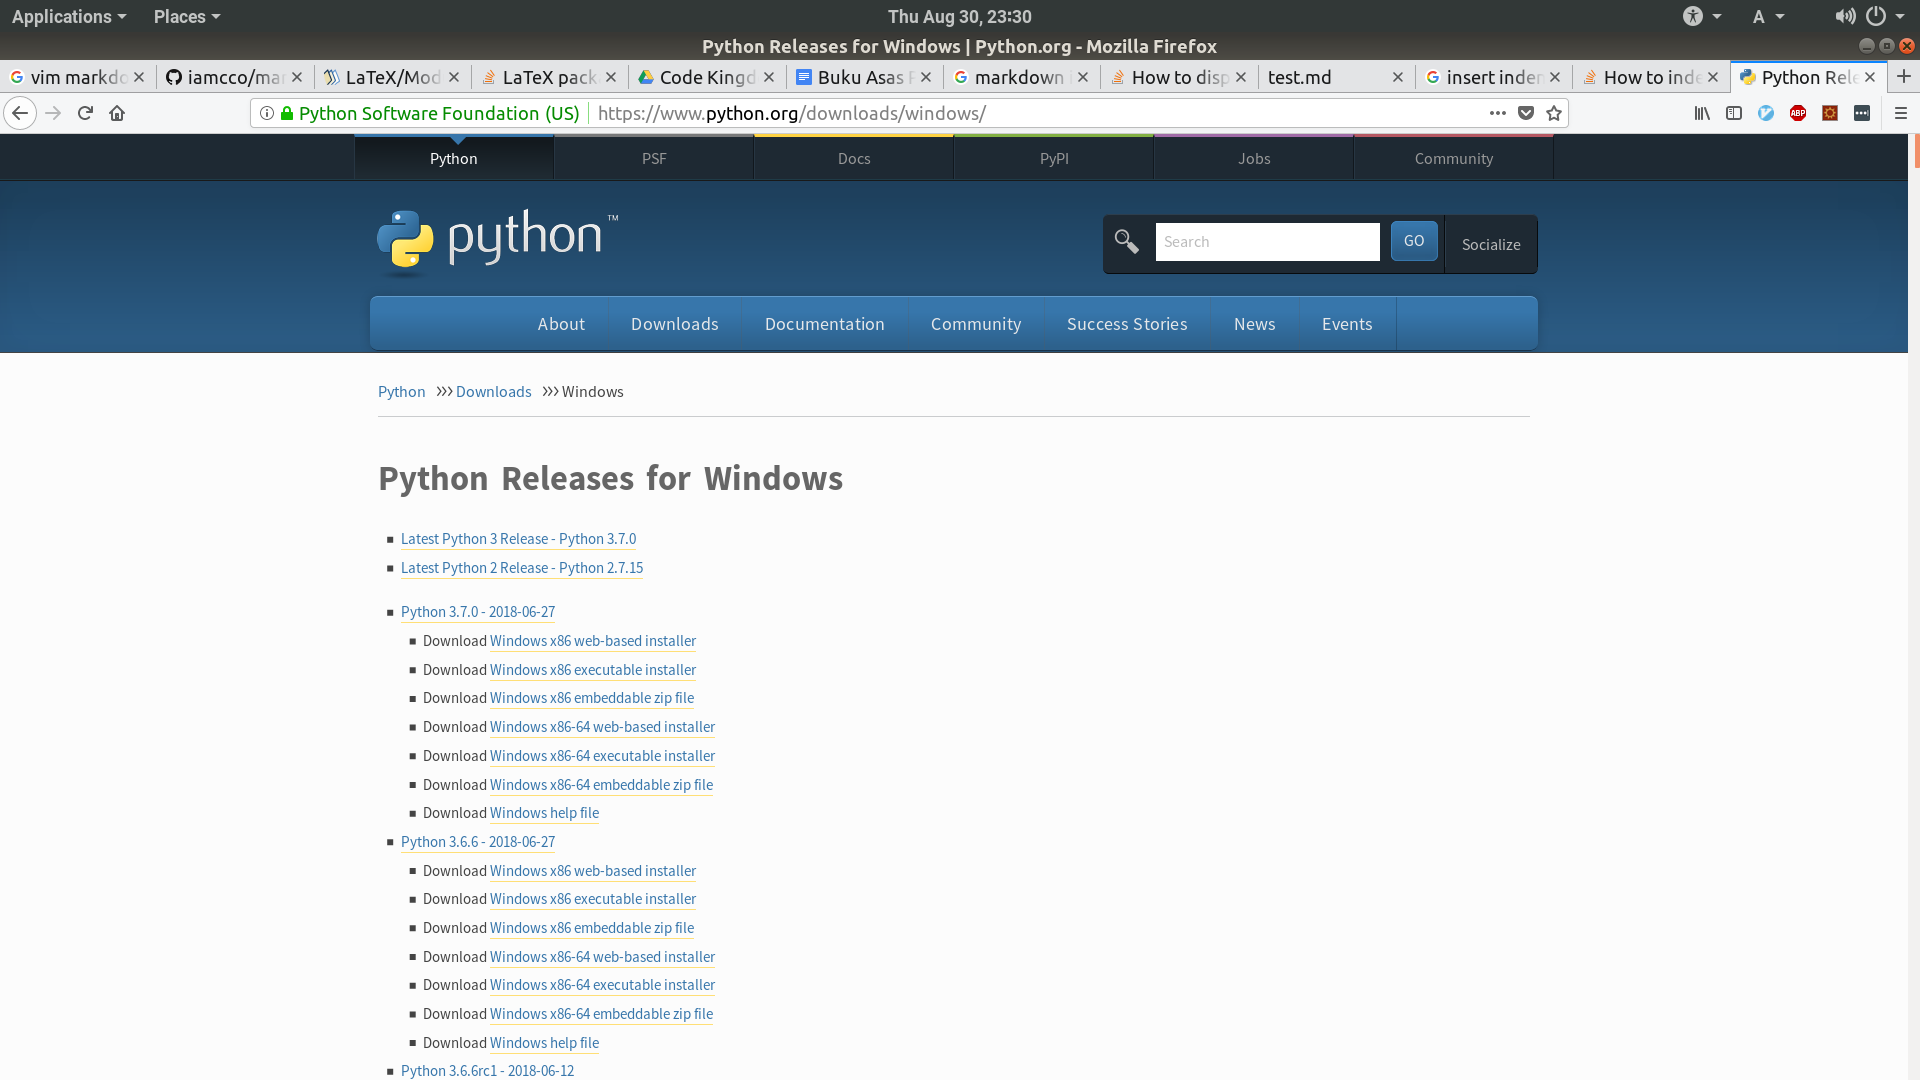
\includegraphics[width=10cm]{./img/1.png}
	\end{figure}

	\item Pilih \textbf{Download Windows} [x86 executable installer] di dalam versi Python yang paling baru dan muat turun
	\item Selepas muat turun, klik dua kali kepada fail yang sudah di muat turun dan mulakan installation Python.
	\item Selepas installation tamat, anda perlu melakukan configuration untuk Enviroment Variable di dalam Windows untuk membolehkan Python di execute di dalam Command Line
	\item PATH sudah di set, dan anda boleh mula Program di dalam Python!

\end{enumerate}

\subsection{}
Cara Install Python di dalam Linux

\paragraph{}
Kebiasaanya, kebanyakan distribution Linux sudah didatangi dengan Python sudah pun siap dipasang. Tetapi, banyak versi Python yang dipasang adalah didalam python versi 2. Untuk memasang python di dalam Linux adalah mudah dengan menggunakan package manager distribution masing-masing. Untuk contoh, buku ini akan menggunakan Ubuntu untuk menunjukkan cara pemasangan Python 3 di dalam Linux.

\begin{enumerate}
	\item Buka terminal anda melalui \textbf{Application} > \textbf{Terminal} 
	\item Taip di terminal command seperti dibawah untuk melihat Python sudah di install di dalam sistem ataupun tidak
		\begin{lstlisting}[language=bash]
$ python --version
Python 3.7.2
		\end{lstlisting}
	\item Guna command di bawah ini untuk install Python di dalam Ubuntu
		\begin{lstlisting}[language=bash]
$ sudo apt update
$ sudo apt upgrade
$ sudo apt install python python-dev
		\end{lstlisting}
\end{enumerate}

\subsection{}
Cara Install Python di dalam Mac

\paragraph{}
Seperti Linux, Mac juga adalah Operating System yang Unix-like yang mempunyai command line tool yang mudah untuk installation python. Dengan mengunakan package manager Homebrew , pengguna Mac dapat membuat installation Python 3 dengan mudah.
Homebrew tidak terdapat secara default di dalam sesuatu komputer Mac , maka buku ini juga akan mengajar sedikit cara untuk menginstall Homebrew di dalam Mac dan menggunakan Homebrew untuk membuat installation Python.

\begin{enumerate}
	\item Buka terminal anda \textbf{Application} > \textbf{Terminal} 
	\item Jika anda sudah mempunyai Homebrew boleh terus melangkah ke step 4 . Jika tidak , install Homebrew dengan mengunakan command di bawah. 
		\begin{lstlisting}[language=bash]
$ ruby -e "$(curl -fsSL https://raw.githubusercontent.com/
Homebrew/install/master/install)"
		\end{lstlisting}
	\item ubah .profile anda dan tambah command di bawah ini supaya boleh mengunakan Homebrew di dalam Terminal. 
		\begin{lstlisting}[language=bash]
export PATH="/usr/local/opt/python/libexec/bin:$PATH"
		\end{lstlisting}
	\item Install Python dengan Homebrew
		\begin{lstlisting}[language=bash]
$ brew install python
		\end{lstlisting}
	\item Semak Python sudah tamat di install 
		\begin{lstlisting}[language=bash]
$ python --version
Python 3.7.2
		\end{lstlisting}

\end{enumerate}
